% !TeX root = ../main.tex
\chapter{Project 03: Secure State Estimation of a Dynamic CPS with Sparse Sensor Attacks}

\section{Objectives}
The aim of this project is to use an online observer in order to estimate the state of the given system un sensor attack, which entitles estimating the states and the attacks at the same time.

\section{Setting of the problem}
The system provided for performing this task is an autonomous LTI system with the following state space representation:

\begin{equation}
	\begin{cases}
		x(k+1) = A x(k) \\
		y(k) = C x(k) + a
	\end{cases}
\end{equation}
where,
\begin{itemize}
	\item the state dimension is $n = 15$
	\item the number of sesors is $q = 30$
	\item the number of sensor under attack $h = 3$
\end{itemize}

It is assumed that attack is going to remain constant for a time-windows, which can be a reasonable assumption having an small enough sampling rate.

\section{Implementation}
\subsection{Luenberg Observer}
The system under the study has a mode equal to 1. According to the proposition of Observability of Dynamic CPSs with constant attacks, If the matrix $A$ has an eigenvalue equal to 1, the dynamic CPS with constant attacks is not observable. Hence, we cannot adopt a Luenberg observer.

\subsection{Sparse Soft Observer (SSO)}
This observer, which is the dynamical version of the ISTA can be adopted in order to perform online secure estimation for a dynamical system. The steps of these iterative algorithm is as follows:

\textbf{Initialization:} \(\tau > 0\), \(\hat{x}(0) \in \mathbb{R}^{n}\), \(\hat{a}(0) \in \mathbb{R}^{q}\), e.g., \(\hat{x}(0) = 0\), \(\hat{a}(0) = 0\)

\textbf{For} \( k = 0, \dots, T_{\max} \),

\begin{align}
    y(k) &= Cx(k) + a(k) \\
    \hat{y}(k) &= C\hat{x}(k) + \hat{a}(k) \\
    \hat{x}(k+1) &= A\hat{x}(k) - \nu A C^\top (\hat{y}(k) - y(k)) \\
    \hat{a}(k+1) &= S_{\nu\lambda} [\hat{a}(k) - \nu (\hat{y}(k) - y(k))] \\
    x(k+1) &= A x(k)
\end{align}

Here, the values of the attack vectors are constant. As it can be seen, in an attack-free case, by considering $L =\nu A C^\top$, the equation which updates the states becomes that of Luenberg observer. Additionally, for $A = I$, the equations turns into ISTA.

The suggested values of hyperparameters for this algorithm are:

\begin{itemize}
	\item $\lambda = 0.1$
	\item $\nu = \frac{0.99}{\|G\|_2^2}$, where $G = (C,\ I)$
\end{itemize} 

However, to enhance the convergence rate, the following hyperparameters are used:
\begin{itemize}
	\item $\lambda = 0.5$
	\item $\nu = \frac{0.99 \times 2}{\|G\|_2^2}$, where $G = (C,\ I)$
\end{itemize} 

\subsection{Deadbeat Sparse Soft Observer (D-SSO)}
This observer is the dynamic counterpart of IJAM algorithm. The steps of this algorithm is as follows:

\textbf{For} \( k = 0, \dots, T_{\max} \),

\begin{align}
    y(k) &= Cx(k) + a(k) \\
    \hat{y}(k) &= C\hat{x}(k) + \hat{a}(k) \\
    \hat{x}(k+1) &= A\hat{x}(k) - L (\hat{y}(k) - y(k)) \\
    \hat{a}(k+1) &= S_{\nu\lambda} [\hat{a}(k) - \nu (\hat{y}(k) - y(k))] \\
    x(k+1) &= A x(k)
\end{align}

Where $L$ is designed such that, $eig(A - LC) = 0$. Also here, the values of the attack vectors are constant. In order not to face numerical issues, the \texttt{place()} command is used by randomized desirable eigenvalues close enough to zero. As it can easily be shown, by setting $L = C^+$ and $A = I$, the algorithm turns into IJAM.

The suggested value of hyperparameters are:
\begin{itemize}
	\item $\lambda = 0.1$
	\item $\nu = 0.7$
\end{itemize} 

However, to enhance the convergence rate, the following hyperparameters are used:
\begin{itemize}
	\item $\lambda = 0.5$
	\item $\nu = 0.9$
\end{itemize} 

Which enjoy a higher value of $\nu$, or a lower inertia, and a higher threshold for soft-thresholding, or a higher value of $\lambda$.

\subsection{Enhancing the estimation by removing the attacked measurements}
In order to obtain a very small value of state estimation error, after the change in the value of the state update becomes smaller than a certain threshold, in this case $\delta = 10^{-10}$ is used. The rows of the matrix C corresponding the attack can be eleminated, by doing so, a higher estimation precision can be obtained.

\section{Analysis}
As it can be seen, the values of the hyperparameters stabilizing ISTA and IJAM are stabilizing also SSO and D-SSO, respectively.

It is observed that both the algorithms are capable of performing secure estimation, estimating the states as well as the attacks and their corresponding positions, in a finite time. 

Since SSO and D-SSO are the dynamic counterparts of ISTA and IJAM, respectively, it is expected that D-SSO output SSO in terms of convergence velocity. The same expectation is that D-SSO represents worst transient performance. In the following figure, both of these observations are depicted.
 
\begin{figure}[H] % h means "here", can also use t (top), b (bottom), p (page)
    \centering
    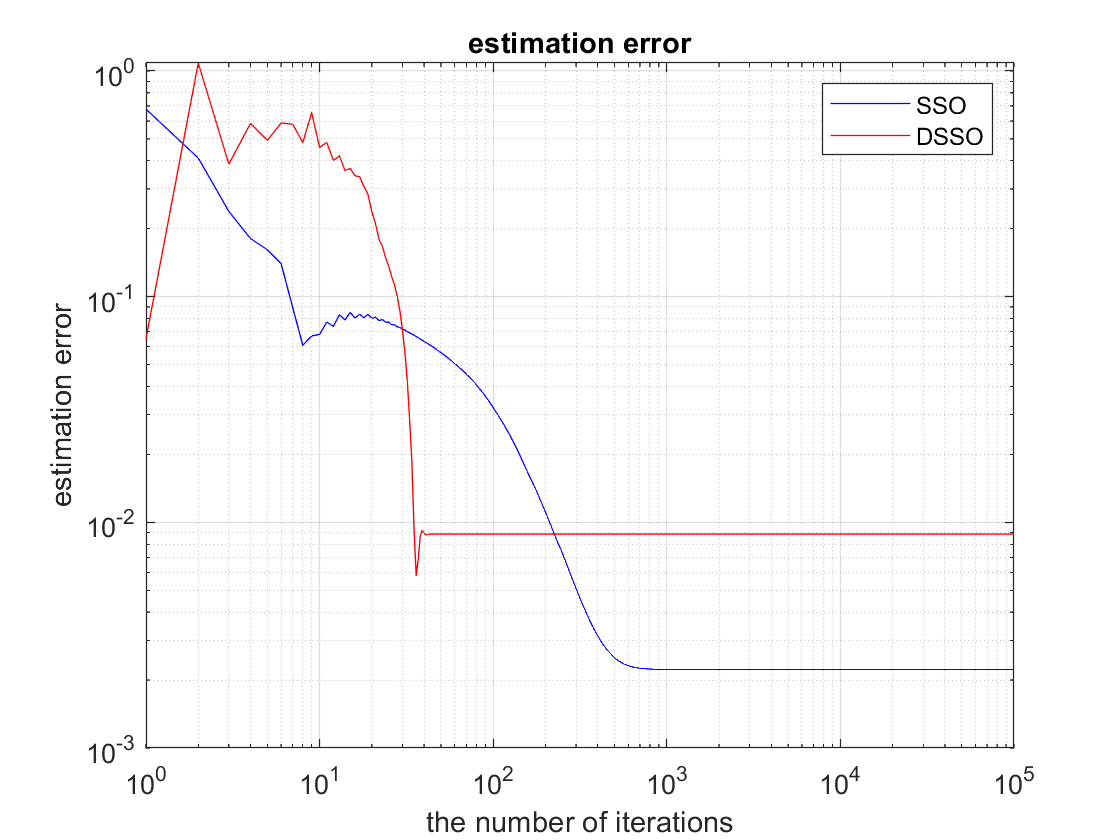
\includegraphics[width=0.75\textwidth]{dynamic_state_error.png} % Adjust width as needed
    \caption{State estimation error of SSO and D-SSO algorithms with suggested values of hyperparameters}
\end{figure}

\begin{figure}[H] % h means "here", can also use t (top), b (bottom), p (page)
    \centering
    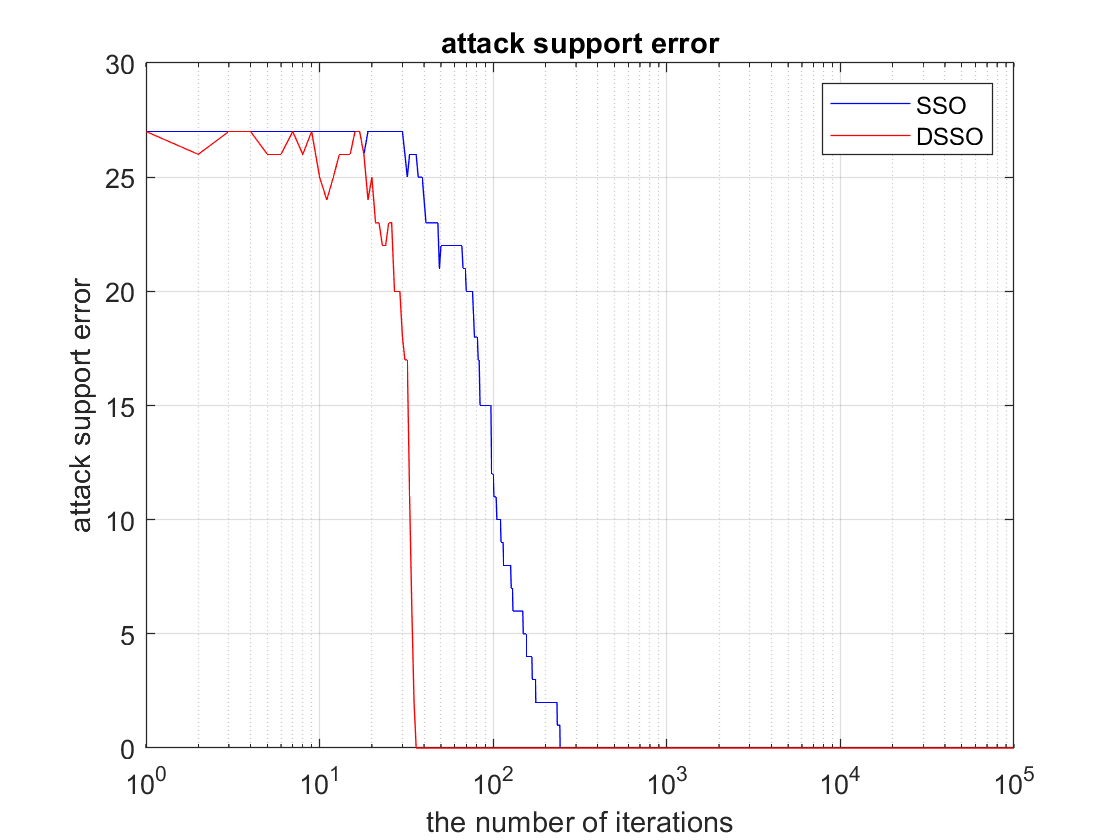
\includegraphics[width=0.75\textwidth]{dynamic_attack_error.png} % Adjust width as needed
    \caption{Attack support error of SSO and D-SSO algorithms with suggested values of hyperparameters}
\end{figure}

Regarding tuning the hyperparameters, it was observed that the following values lead to a way faster results:
For SSO:
\begin{itemize}
	\item $\lambda = 0.1$
	\item $\nu = 0.7$
\end{itemize} 
For D-SSO:
\begin{itemize}
	\item $\lambda = 0.5$
	\item $\nu = 0.9$
\end{itemize} 
Which enjoy a higher value of $\nu$, or a lower inertia, and a higher threshold for soft-thresholding, or a higher value of $\lambda$.

\begin{figure}[H] % h means "here", can also use t (top), b (bottom), p (page)
    \centering
    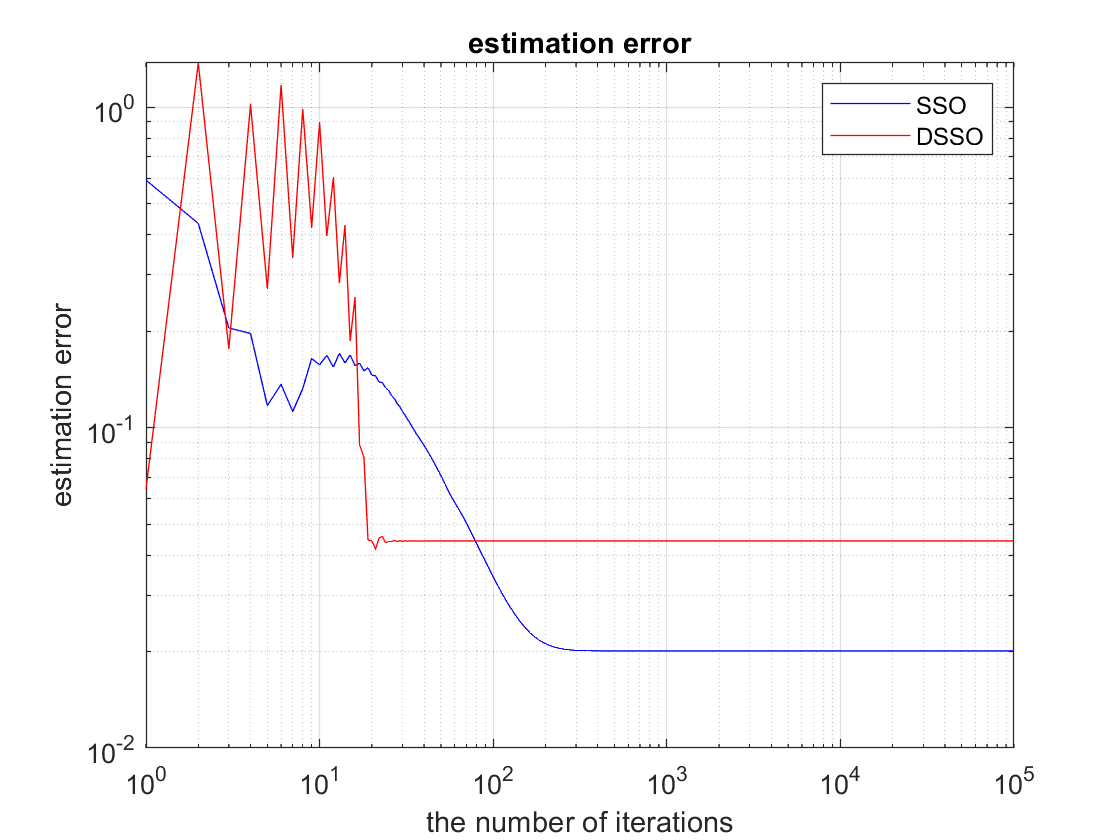
\includegraphics[width=0.75\textwidth]{dynamic_attack_error_modified.png} % Adjust width as needed
    \caption{State estimation error of SSO and D-SSO algorithms with modified values of hyperparameters}
\end{figure}

\begin{figure}[H] % h means "here", can also use t (top), b (bottom), p (page)
    \centering
    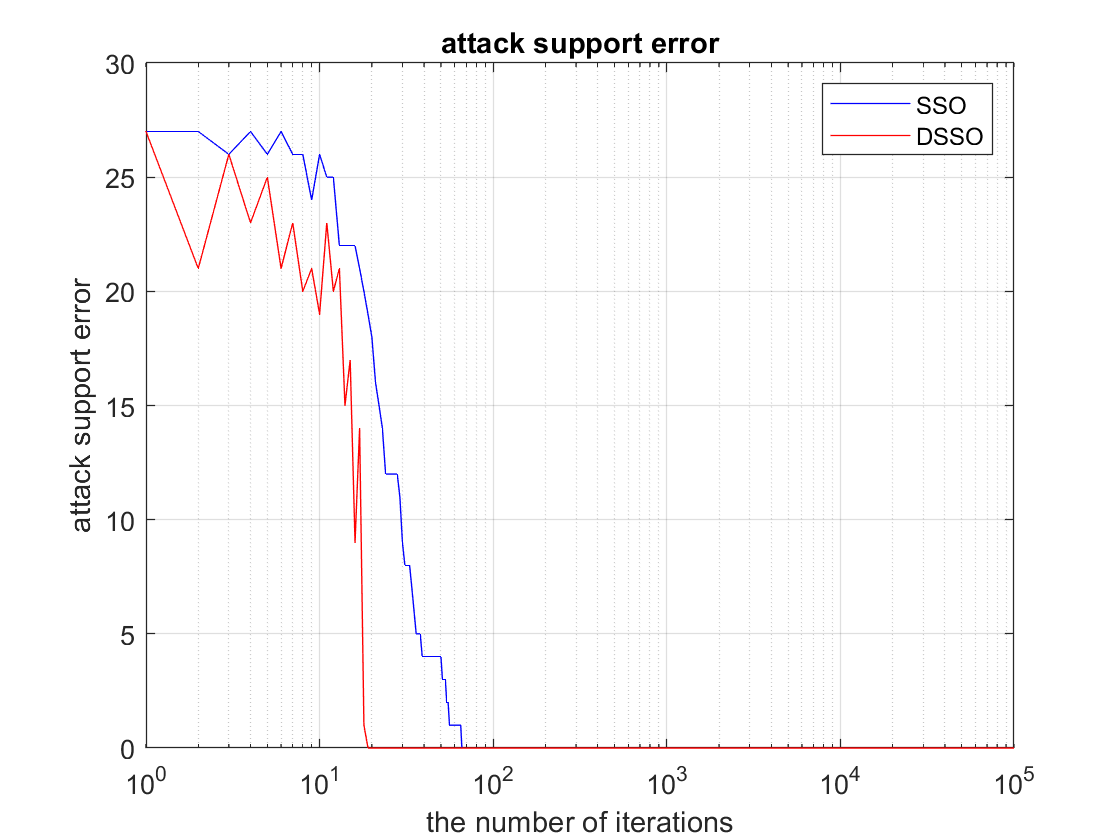
\includegraphics[width=0.75\textwidth]{dynamic_attack_error_modified_2.png} % Adjust width as needed
    \caption{Attack support error of SSO and D-SSO algorithms with modified values of hyperparameters}
\end{figure}

As to enhancing the precision of the estimation, having removed the rows in $C$ corresponding to the attack, an almost zero error was obtained.

\begin{figure}[H] % h means "here", can also use t (top), b (bottom), p (page)
    \centering
    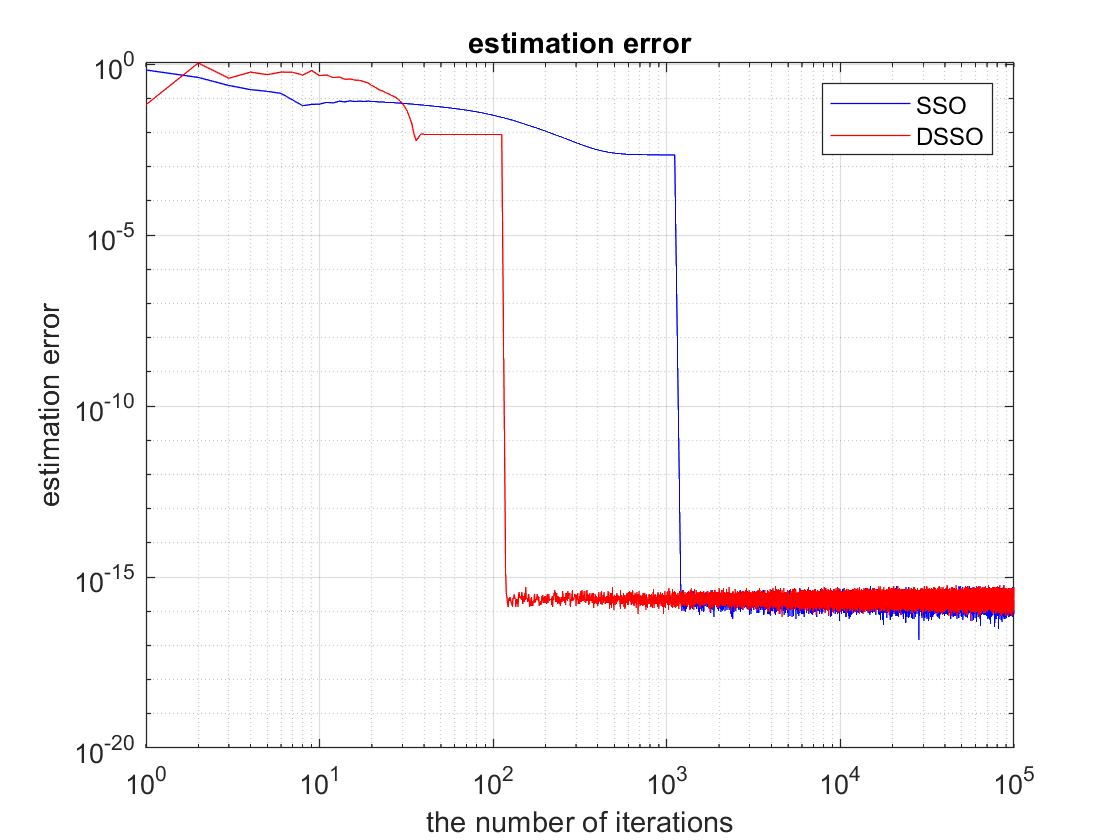
\includegraphics[width=0.75\textwidth]{dynamic_zero_error.png} % Adjust width as needed
    \caption{State estimation error of SSO and D-SSO algorithms with putting aside the sensors under the attack, after correctly estimating the position of the attacks.}
\end{figure}

It can be seen that after convergence, the input of the observer itself introduces high-frequency oscillations. In order to modify this unwanted behavior, the input of the observer is applied only if its inovation is larger than the precision of the sensor; in this case, $10^{-8}$ is considered. The result is going to be as follows:


\begin{figure}[H] % h means "here", can also use t (top), b (bottom), p (page)
    \centering
    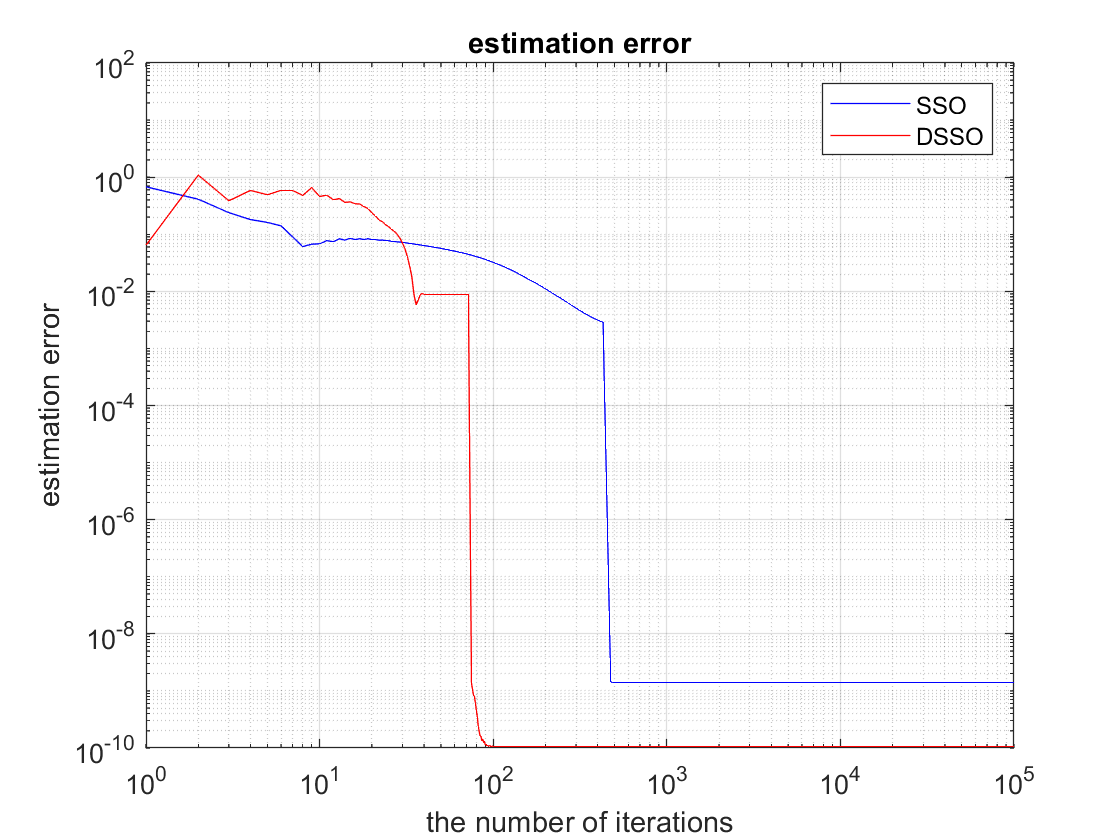
\includegraphics[width=0.75\textwidth]{dynamic_zero_error_clean.png} % Adjust width as needed
    \caption{State estimation error of SSO and D-SSO algorithms with putting aside the sensors under the attack, and cutting the input of the observer when their inovation is smaller than the precision of the sensor.}
\end{figure}
 
\section{conclusion}
It was observed that SSO and D-SSO are capable of secure state estimation of dynamical CPSs under constant values of attacks in finite amount of time. 

Further it was observed that having estimated the position of the attacks, by putting aside the tampered data comming from the attacked sensors, an almost zero estimation error can be obtained. However, in this case, a high-frequency oscillation is introduced due to numerical errors. In order to remove this, the input of the observer is not applied to modify the dynamic of the observer if the difference of the measurements and the system model is smaller than the precision of the sensors.











